% Options for packages loaded elsewhere
\PassOptionsToPackage{unicode}{hyperref}
\PassOptionsToPackage{hyphens}{url}
%
\documentclass[
  12pt,
]{article}
\usepackage{lmodern}
\usepackage{amssymb,amsmath}
\usepackage{ifxetex,ifluatex}
\ifnum 0\ifxetex 1\fi\ifluatex 1\fi=0 % if pdftex
  \usepackage[T1]{fontenc}
  \usepackage[utf8]{inputenc}
  \usepackage{textcomp} % provide euro and other symbols
\else % if luatex or xetex
  \usepackage{unicode-math}
  \defaultfontfeatures{Scale=MatchLowercase}
  \defaultfontfeatures[\rmfamily]{Ligatures=TeX,Scale=1}
  \setmainfont[]{Times New Roman}
\fi
% Use upquote if available, for straight quotes in verbatim environments
\IfFileExists{upquote.sty}{\usepackage{upquote}}{}
\IfFileExists{microtype.sty}{% use microtype if available
  \usepackage[]{microtype}
  \UseMicrotypeSet[protrusion]{basicmath} % disable protrusion for tt fonts
}{}
\usepackage{xcolor}
\IfFileExists{xurl.sty}{\usepackage{xurl}}{} % add URL line breaks if available
\IfFileExists{bookmark.sty}{\usepackage{bookmark}}{\usepackage{hyperref}}
\hypersetup{
  pdftitle={Assessing water level changes from hurricanes from 2000 - 2020},
  pdfauthor={Camila Zarate Ospina, Savannah Artusi, and Autumn Dunn},
  hidelinks,
  pdfcreator={LaTeX via pandoc}}
\urlstyle{same} % disable monospaced font for URLs
\usepackage[margin=2.54cm]{geometry}
\usepackage{longtable,booktabs}
% Correct order of tables after \paragraph or \subparagraph
\usepackage{etoolbox}
\makeatletter
\patchcmd\longtable{\par}{\if@noskipsec\mbox{}\fi\par}{}{}
\makeatother
% Allow footnotes in longtable head/foot
\IfFileExists{footnotehyper.sty}{\usepackage{footnotehyper}}{\usepackage{footnote}}
\makesavenoteenv{longtable}
\usepackage{graphicx,grffile}
\makeatletter
\def\maxwidth{\ifdim\Gin@nat@width>\linewidth\linewidth\else\Gin@nat@width\fi}
\def\maxheight{\ifdim\Gin@nat@height>\textheight\textheight\else\Gin@nat@height\fi}
\makeatother
% Scale images if necessary, so that they will not overflow the page
% margins by default, and it is still possible to overwrite the defaults
% using explicit options in \includegraphics[width, height, ...]{}
\setkeys{Gin}{width=\maxwidth,height=\maxheight,keepaspectratio}
% Set default figure placement to htbp
\makeatletter
\def\fps@figure{htbp}
\makeatother
\setlength{\emergencystretch}{3em} % prevent overfull lines
\providecommand{\tightlist}{%
  \setlength{\itemsep}{0pt}\setlength{\parskip}{0pt}}
\setcounter{secnumdepth}{5}
\usepackage{booktabs}
\usepackage{longtable}
\usepackage{array}
\usepackage{multirow}
\usepackage{wrapfig}
\usepackage{float}
\usepackage{colortbl}
\usepackage{pdflscape}
\usepackage{tabu}
\usepackage{threeparttable}
\usepackage{threeparttablex}
\usepackage[normalem]{ulem}
\usepackage{makecell}
\usepackage{xcolor}

\title{Assessing water level changes from hurricanes from 2000 - 2020}
\usepackage{etoolbox}
\makeatletter
\providecommand{\subtitle}[1]{% add subtitle to \maketitle
  \apptocmd{\@title}{\par {\large #1 \par}}{}{}
}
\makeatother
\subtitle{Web address for GitHub repository:
\url{https://github.com/Autumn41/Dunn-Artusi-Zarate_ENV872_Project.git}}
\author{Camila Zarate Ospina, Savannah Artusi, and Autumn Dunn}
\date{}

\begin{document}
\maketitle

\newpage
\tableofcontents 
\newpage
\listoftables 
\newpage
\listoffigures 
\newpage

\hypertarget{rationale-and-research-questions}{%
\section{Rationale and Research
Questions}\label{rationale-and-research-questions}}

From 2000 to 2020, North Carolina was hit with 64 hurricanes and 26 of
those hurricanes occurred in September. With climate change, hurricanes
are expected to occur more frequently and at higher intensity (Elsner,
2006). Higher intensity storms will likely cause flooding of cities and
urban areas which many infrastructures are not designed to accommodate
(James et al., 2020; Marsooli \& Lin, 2020). Additionally, much of North
Carolina Piedmont wetlands have been drained and many streams are
degraded due to urban disturbances (Carle, 2011; Violin et al., 2011).
Wetlands and streams are natural systems that store flood water, and
without them, many areas that have not flooded in the past will be at
risk (Ameli \& Creed, 2019). Based on National Climatic Data Center
Event Report for Hurricanes, in 2018, 46 people died due to hurricane
Florence and Michael, the only two hurricanes to hit that year and in
2016, 28 people died due to hurricane Matthew. From 2000 - 2012, 41
people in total died due to hurricanes. Death from hurricanes are
usually linked to flooding, which can cause expose individuals to sewage
water, damage infrastructure making roads and homes dangerous, and
potentially drown victims (Choudhary et al., 2012). Investing in
pre-disaster hazard mitigation has been shown to be economically
beneficial and save lives (Villa, 2020). In order to update
infrastructure, expected water input and time period of elevated water
levels are needed. Using stream gage height, we selected Yadkin River,
Mills River, and French Broad River, because of their location along the
path of Hurricane Florence, which hit North Carolina in September of
2018 (Figure 1). We focused on two questions: has gage height changed
over 2000-2020 for September from hurricanes, and are gage heights
significantly different between 2001 and 2018?

\begin{figure}
\centering
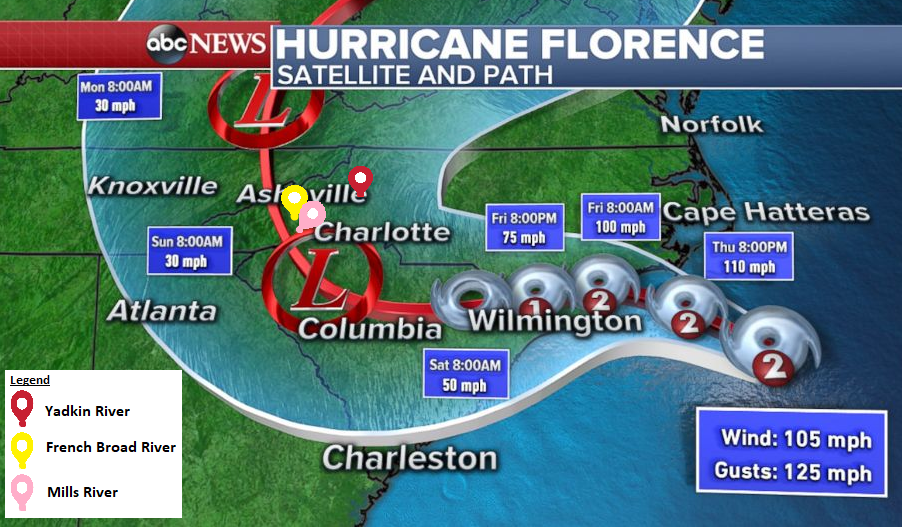
\includegraphics[width=\textwidth,height=0.4\textheight]{../Analysis/Hurricane_Path_Sites.png}
\caption{Hurricane Florence path in North Carolina, including selected
river sites.}
\end{figure}

\clearpage

\hypertarget{dataset-information}{%
\section{Dataset Information}\label{dataset-information}}

Data were retrieved from USGS National Water Information. USGS uses an
eight digit code for each site (listed below). The parameter of
interest, represented as GH in the tables, was gage height (feet),
identified using the pcode 00065. Daily mean value was used, using the
scode 00003.

\begin{longtable}[]{@{}lll@{}}
\caption{Site locations and site codes.}\tabularnewline
\toprule
River Names & NC City & Site Code\tabularnewline
\midrule
\endfirsthead
\toprule
River Names & NC City & Site Code\tabularnewline
\midrule
\endhead
Yadkin River & Patterson & 02111000\tabularnewline
Mills River & Mills River & 03446000\tabularnewline
French Broad River & Fletcher & 03447687\tabularnewline
\bottomrule
\end{longtable}

To process the data, gage heights for September for all available years
were selected from the raw gage height data. This was done by converting
the raw date to a recognized date format and filtering by month. Later,
to run the t-tests, each river dataset was subsetted into two datasets,
one for 2001 and one for 2018 for each river.

\newpage

\hypertarget{exploratory-analysis}{%
\section{Exploratory Analysis}\label{exploratory-analysis}}

The Yadkin River gage height for September for every year from 2000 -
2020. This shows the gage height variation, and higher values and more
spread in the data indicate flooding, likely from hurricanes. Years that
had the most spread and highest values were 2004 and 2018.

\begin{figure}
\centering
\includegraphics{ZarateArtusiDunn_ENV872_Project_files/figure-latex/Figure2-1.pdf}
\caption{Yadkin Gage Height as points on individual plots for September}
\end{figure}

\newpage

The Mills River gage height for September for every year from 2000 -
2020. This shows the gage height variation, and higher values and more
spread in the data indicate flooding, likely from hurricanes. Years that
had the most spread and highest values were 2004 and 2009.

\begin{figure}
\centering
\includegraphics{ZarateArtusiDunn_ENV872_Project_files/figure-latex/Figure3-1.pdf}
\caption{Mills Gage Height as points on individual plots for September}
\end{figure}

\newpage

The French Broad River gage height for September for every year from
2000 - 2020. This shows the gage height variation, and higher values and
more spread in the data indicate flooding, likely from hurricanes. Years
that had the most spread and highest values were 2004, 2009, and 2020.

\begin{figure}
\centering
\includegraphics{ZarateArtusiDunn_ENV872_Project_files/figure-latex/Figure4-1.pdf}
\caption{French Broad Gage Height as points on individual plots for
September}
\end{figure}

\newpage

A necessary assumption for statistical t-tests is that variances are
approximately equal for both study samples, with the ratio of variances
produced using the var.test function at around 0.5. This assumption was
not met in comparing the 2001 to 2018 samples for some of the rivers.
Yadkin River was especially low (0.07) and French Broad River was 0.36.
The ratio for Mills River was appropriate (0.44). Another necessary
assumption is that the data are normally distributed, which was again
not the case for all three rivers in both years (Figure 5). All samples
were notably right-skewed; however, this makes sense given that gage
heights are expected to remain around the same level. The high values
that are skewing the distribution of the data could reflect the
increases in gage height due to hurricanes (especially in 2018) or other
unusual events (for example, human regulation of river flow).

\begin{figure}
\centering
\includegraphics{ZarateArtusiDunn_ENV872_Project_files/figure-latex/Figure5-1.pdf}
\caption{Histograms of Yadkin, French Broad, and Mills River gage
heights in September 2001 and 2018.}
\end{figure}

\newpage

\hypertarget{analysis}{%
\section{Analysis}\label{analysis}}

To answer question 1, we performed a time series with the objective to
identify if gage heights have changed in September over the last 20
years. The results from the test can be seen in Table 2.

\begin{table}

\caption{\label{tab:ResultsTable1}Results from the Mann-Kendall test}
\centering
\begin{tabular}[t]{l|r|l}
\hline
River Name & Tau Score & P-Value\\
\hline
Yadkin & 0.13591 & < 2.22e-16\\
\hline
Mills & 0.13591 & < 2.22e-16\\
\hline
French Broad & 0.15523 & < 2.22e-16\\
\hline
\end{tabular}
\end{table}

To answer question 2, we performed a t-test with the objective to
identify if the gage heights between 2001 (out baseline year) and 2018
(the year when Hurricane Florence impacted North Carolina) were
statistically different. The results from the test can be seen in Table
3.

\begin{table}

\caption{\label{tab:ResultsTable2}Results from the T-test}
\centering
\begin{tabular}[t]{|>{}l|||>{}r|||>{}r|||>{}r|||>{}r|||>{}r|}
\hline
River Name & 2001 Avg GH & 2018 Avg GH & var.test & T-Stat & P-Value\\
\hline
Yadkin & 1.00 & 1.49 & 0.07 & -6.22 & 6.00e-08\\
\hline
Mills & 1.80 & 2.08 & 0.44 & -5.37 & 1.46e-06\\
\hline
French Broad & 4.12 & 5.40 & 0.36 & -6.72 & 1.00e-08\\
\hline
\end{tabular}
\end{table}

\hypertarget{question-1-has-gage-height-changed-over-2000-2020-for-september-from-hurricanes}{%
\subsection{Question 1: Has gage height changed over 2000-2020 for
September from
hurricanes?}\label{question-1-has-gage-height-changed-over-2000-2020-for-september-from-hurricanes}}

Yadkin River, Mills River, and French Broad River had a significant
(p-value \textless{} 0.05) monotonic upward trend. French Broad River
had the largest upward trend (0.155) and Yadkin River and Mills River
had the smallest upward trend (0.136). With these results, we reject the
null hypothesis and conclude that gage Height has changed in September
over the last 20 years and that this change is statistically significant
for all three rivers.

\hypertarget{question-2-are-gage-heights-significantly-different-between-2001-and-2018}{%
\subsection{Question 2: Are gage heights significantly different between
2001 and
2018?}\label{question-2-are-gage-heights-significantly-different-between-2001-and-2018}}

The mean gage heights for each river was higher in 2018 than in 2001,
and these differences were statistically significant (distribution of
gage heights shown in Figure 6). Since the t-statistic for the Yadkin,
Mills, and French Broad Rivers (-6.22, -5.37, and -6.72) are negative,
this indicates that the 2018 gage heights are greater than the 2001
heights. The Yadkin River gage was 0.49 feet higher in 2018 (p-value
\textless{} 0.05). The Mills River gage was 0.28 feet higher in 2018
(p-value \textless{} 0.05). The French Broad River gage was 1.28 feet
higher in 2018 (p-value \textless{} 0.05). With these results, we reject
the null hypothesis and conclude that the average gage heights for 2001
and 2018 are different and that this difference is statistically
significant for all three rivers.

\begin{figure}
\centering
\includegraphics{ZarateArtusiDunn_ENV872_Project_files/figure-latex/Figure6-1.pdf}
\caption{Gage height box plots for Yadkin, French Broad, and Mills River
in September 2001 versus 2018.}
\end{figure}

\newpage

\hypertarget{summary-and-conclusions}{%
\section{Summary and Conclusions}\label{summary-and-conclusions}}

Water level has been increasing for the month of September over the last
20 years, based on the significant upward trend from the time series
analysis. Though storms appeared to have decreased in frequency (there
were 48 storms from 2000 - 2010, but only 18 storms from 2011 -- 2020)
it is evident that the severity of the storms has increased, based on
both deaths and increasing water levels. Further research should be done
to quantify how much additional water is deposited per storm and what
updates to infrastructure should be done to account for this additional
water.

To evaluate increases in hurricane intensity due to climate change, we
compared gage heights between 2001, a year with no September hurricanes
impacting North Carolina, and 2018, a year with the major Hurricane
Florence. The results of our t-test showed that there was a significant
difference in gage height, indicating that hurricane intensity and flood
potential increased. While it is possible that other factors contributed
to this increase in gage height, our conclusions are supported by
existing research studies that link climate change to increases in
hurricane intensity (Emanuel, 1987). However, most of the data used for
our t-tests failed to satisfy the assumptions of equal variances and
normality. Future, more in-depth studies should transform and normalize
the data, or use a different statistical test that accounts for these
failed assumptions.

\newpage

\hypertarget{references}{%
\section{References}\label{references}}

\setlength{\parindent}{-0.2in}
\setlength{\leftskip}{0.2in}
\setlength{\parskip}{8pt}

\noindent

Ameli, A. A., \& Creed, I. F. (2019). Does Wetland Location Matter When
Managing Wetlands for Watershed-Scale Flood and Drought Resilience?
Journal of the American Water Resources Association, 55(3), 529--542.
\url{https://doi.org/10.1111/1752-1688.12737}

Carle, M. V. (2011). Estimating wetland losses and gains in coastal
north carolina: 1994-2001. Wetlands, 31(6), 1275--1285.
\url{https://doi.org/10.1007/s13157-011-0242-z}

Choudhary, E., Zane, D. F., Beasley, C., Jones, R., Rey, A., Noe, R. S.,
Martin, C., Wolkin, A. F., \& Bayleyegn, T. M. (2012). Evaluation of
active mortality surveillance system data for monitoring
hurricane-related deaths-texas, 2008. Prehospital and Disaster Medicine,
27(4), 392--397. \url{https://doi.org/10.1017/S1049023X12000957}

Elsner, J. B. (2006). Evidence in support of the climate change-Atlantic
hurricane hypothesis. Geophysical Research Letters, 33(16), 1--3.
\url{https://doi.org/10.1029/2006GL026869}

Emanuel, K. A. (1987). The dependence of hurricane intensity on climate.
Nature, 326, 483--485. \url{https://doi.org/10.1038/326483a0}

James M. Shultz, Ph.D., Duane E. Sands, M.D., James P. Kossin, Ph.D.,
and Sandro Galea, M.D., Dr.~P. H. (2020). Double Environmental Injustice
- Climate Change, Hurricane Dorian, and the Bahamas. The New England
Journal of Medicine, 1--3.

Marsooli, R., \& Lin, N. (2020). Impacts of climate change on hurricane
flood hazards in Jamaica Bay, New York. Climatic Change, 163(4),
2153--2171. \url{https://doi.org/10.1007/s10584-020-02932-x}

Villa, Clifford, et al.~Environmental Justice: Law, Policy \&
Regulation. Carolina Academic Press, 2020.

Violin, C. R., Cada, P., Sudduth, E. B., Hassett, B. A., Penrose, D. L.,
\& Bernhardt, E. S. (2011). Effects of urbanization and urban stream
restoration on the physical and biological structure of stream
ecosystems. Ecological Applications, 21(6), 1932--1949.
\url{https://doi.org/10.1890/10-1551.1}

\end{document}
